%% General definitions
\documentclass{article} %% Determines the general format.
\usepackage{a4wide} %% paper size: A4.
\usepackage[utf8]{inputenc} %% This file is written in UTF-8.
%% Some editors on Windows cannot save files in UTF-8.
%% If there is a problem with special characters not showing up
%% correctly, try switching "utf8" to "latin1" (ISO 8859-1).
\usepackage[T1]{fontenc} %% Format of the resulting PDF file.
\usepackage{fancyhdr} %% Package to create a header on each page.
\usepackage{lastpage} %% Used for "Page X of Y" in the header.
                      %% For this to work, you have to call pdflatex twice.
\usepackage{enumerate} %% Used to change the style of enumerations (see below).

\usepackage{amssymb} %% Definitions for math symbols.
\usepackage{amsmath} %% Definitions for math symbols.

\usepackage{tikz}  %% Pagacke to create graphics (graphs, automata, etc.)
\usetikzlibrary{automata} %% Tikz library to draw automata
\usetikzlibrary{arrows}   %% Tikz library for nicer arrow heads

\usepackage{hyperref} %% hyperlinks

%% Left side of header
\lhead{\course\\\semester\\Exercise \homeworkNumber}
%% Right side of header
\rhead{\authorname\\Page \thepage\ of \pageref{LastPage}}
%% Height of header
\usepackage[headheight=36pt]{geometry}
%% Page style that uses the header
\pagestyle{fancy}

\newcommand{\authorname}{Benjamin Regez\\Luis Tritschler}
\newcommand{\semester}{Spring Semester 2026}
\newcommand{\course}{Foundations of Artificial Intelligence}
\newcommand{\homeworkNumber}{3}

\renewcommand{\thesection}{Exercise \homeworkNumber.\arabic{section}}


\begin{document}

\section{}
\begin{enumerate}[(a)]
    \item \textit{A state space that contains cycles but where
    tree search is still guaranteed to terminate.} \\[0.5em]
    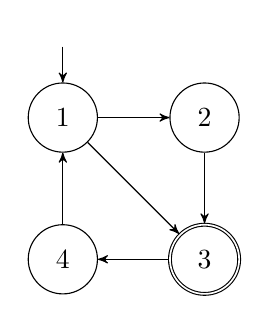
\begin{tikzpicture}[->,>=stealth',auto,node distance=1.8cm]
        \node[initial above, initial text=, state] (1) {1};
        \node[state] (2) [right of=1] {2};
        \node[state, accepting] (3) [below of=2] {3};
        \node[state] (4) [left of=3] {4};
        \path (1) edge node {} (2);
        \path (2) edge node {} (3);
        \path (3) edge node {} (4);
        \path (4) edge node {} (1);
        \path (1) edge node {} (3);
    \end{tikzpicture}
    \item \textit{A state space where the optimal expansion
    order for graph search results in fewer expansions than
    the optimal expansion order for tree search.}\\[0.5em]
    Such a state space cannot exist. We will show this by
    direct proof:\\[0.3em]
    Let $S$ be an arbitrary state space with at least one
    solution for $\mathcal{S}$. Then, the optimal expansion
    order for tree search from the initial state $s_I$ to
    the nearest reachable goal state $s_G$ will follow the
    shortest path $\pi_{\text{min}}$, i.e., the path with the smallest
    number of $n$ states between $s_I$ and $s_G$. In this
    optimal case, the number of expansions will be $n+1$.
    The latter follows from the premise of optimality: The
    algorithm always chooses to expand to the next node
    with the next state of $\pi_{\text{min}}$.\\[0.3em]
    The only difference in graph search compared to tree search
    is that it has a FIFO queue for states and therefore
    it expands layer by layer. For corner cases (e.g. if
    every expansion layer consist of exactly one node order
    the goal state is in layer 0 or 1), the same path
    $\pi_{\text{min}}$ might be chosen as expansion order.
    In all other cases, more than $n$ nodes are expanded.
    That is, graph search has at least the same amount of
    expansions as tree search, but there is no possibility
    to have less expansions since there is no shorter path
    than $\pi_{\text{min}}$.
    \item \textit{A state space where tree search and graph
    search expand the same amount of nodes (when using the
    same expansion strategy). For this task, your state space
    must have at least 5 states reachable from the initial
    state (including the initial state itself) and every
    solution must have at least length 2.}\\[0.3em]
    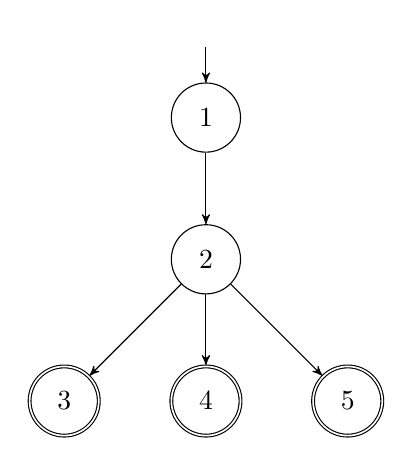
\begin{tikzpicture}[->,>=stealth',auto,node distance=1.8cm]
        \node[initial above, initial text=, state] (1) {1};
        \node[state] (2) [below of=1] {2};
        \node[state, accepting] (4) [below of=2] {4};
        \node[state, accepting] (3) [left of=4] {3};
        \node[state, accepting] (5) [right of=4] {5};
        \path (1) edge node {} (2);
        \path (2) edge node {} (3);
        \path (2) edge node {} (4);
        \path (2) edge node {} (5);
    \end{tikzpicture}
\end{enumerate}

\section{}

\section{}

\section*{Statement on scientific integrity}
\begin{itemize}
    \item In task 3.1(c), ChatGPT was used to ask the
    following question:\\[0.3em]
    \textit{
        Do all states always have the same number of outgoing
        transitions? Or could, for example, one state have two
        transitions to other states and another state only one
        outgoing transition?
    }\\[0.3em] (According to ChatGPT, different numbers
    of outgoing transitions are allowed.)
    \item Google Translate was used to help translate from
    German to English when formulating the answers (individual
    words or phrases - not entire sentences)
\end{itemize}
Appart from the listing above, we did the entire exercise
on our own.

\end{document}
